To address the scarcity of large-scale multi-sensor image-text datasets in \ac{RS}, we introduce \bentxt{}, which comprises co-registered \ac{S1} and \ac{S2} images with semantically rich natural-language annotations relevant for 15 tasks across 4 broad categories: i)~captioning; ii)~binary and iii)~multiple-choice \ac{VQA}; and iv)~\genDet. The co-registered \ac{S1} and \ac{S2} images in \bentxt{} are taken from BigEarthNet~v2.0~\cite{clasen2025reben}, which comprises \num{549488} pairs of \ac{S1} and \ac{S2} images acquired over ten European countries. Each pair is accompanied by a pixel-level \ac{LULC} reference map based on the \ac{CLC} 2018 product  (\texttt{V2020\_20u1})~\cite{clcbook}. Some images in BigEarthNet~v2.0 are partly covered by seasonal snow, clouds, and cloud shadows, and also associated with reference maps containing unclassified pixels (with no LULC label). To construct our dataset, we filter out such image pairs, resulting in \num{464044} co-registered \ac{S1} and \ac{S2} images. In the following, we describe in detail our annotation generation pipeline, present the caption statistics and then finally introduce our \bench{}.  

\subsection{Annotation Generation Pipeline}
The textual annotations for \bentxt{} are generated through a three-stage pipeline (template-based caption generation, \ac{LLM}-based linguistic augmentation, \ac{VQA} and \ac{LULC} annotation generation). 
An overview of the caption generation and linguistic augmentation stage is given in \cref{fig:caption_generation_process}.
\paragraph{Template-based caption generation.} We first construct captions by extracting four categories of spatial attributes directly from the reference maps: the \textit{presence} of \ac{LULC} classes, the \textit{count} of individual contiguous regions per class (instances), the \textit{size} of each class in total and per instance, and pairwise spatial \textit{adjacency} between classes. 
Area values are rounded to the nearest \SI{1000}{\meter\squared} to reduce label noise. 
Classes are assigned to one of three tiers based on their image coverage:
i)~\textit{primary} (> \SI{25}{\percent}); 
ii)~\textit{secondary} (\SI{5}{\percent} - \SI{25}{\percent}); or
iii)~\textit{marginal} (<\SI{5}{\percent}).
Captions are composed from pre-defined templates that contain classes, sizes, and adjacency relations accordingly. 
Each caption is further grounded in spatio-seasonal context by appending the acquisition season, country, and Köppen-Geiger climate zone~\cite{beckHighresolution1Km2023}, derived from high-resolution climate maps.

\paragraph{LLM-based linguistic augmentation.} Although template-based captions guarantee factual correctness, they exhibit limited linguistic variety. 
Therefore, we apply a two-stage augmentation using the quantized Llama-4-Scout-17B model~\cite{touvron2023llamaopenefficientfoundation}.
First, a \textit{paraphrasing} step diversifies lexical and syntactic structure while prohibiting the addition of unsupported information.
Second, a \textit{self-refinement} step \cite{self-refinement} revises the paraphrased output against the original template to eliminate hallucinated content and restore missing information. 
To further increase valid lexical variation, the prompt includes the \ac{CLC} nomenclature, permitting semantically valid substitutions (\eg referring to \emph{Urban fabric} collectively as \emph{Artificial surfaces}). 
Manual evaluation of \num{3209} randomly sampled augmented captions against four binary criteria (linguistic correctness, factual accuracy, completeness, and absence of generation artifacts) yields an average correctness of \SI{93.76}{\percent}, with \SI{77.50}{\percent} of captions satisfying all four criteria simultaneously.
\begin{figure*}[!ht]
    \centering

    \begin{tikzpicture}        
        \node[inner sep=0pt,minimum size=0pt] (CaptionAnchor) at (-4.7, 0) {};
        \node[single arrow,
              minimum height=40mm, minimum width=20mm,
              single arrow head extend=2mm,
              anchor=west, rotate=-90, fill=gray!15] at (1.33,-4) {};
        \node[anchor=west] (refMap) at (0,0)
            {
\includegraphics[width=\BenImgWidth]{figures/dataset/samples/_ref_map_S2A_MSIL2A_20170818T103021_N9999_R108_T32TMT_61_44.png}};
        \node[anchor=south] (refMapCap) at ($(refMap.north) + (0,-.2)$) {\small\textcolor{gray}{Reference map}};

        \node[align=justify, anchor=south east, text width=30mm, minimum width=30mm, minimum height=20mm, fill=cyan!20, rounded corners=2mm, font=\scriptsize] (PresenceSizeTemplate) at ($(refMap.north west) + (-.2,.2)$) {This image primarily shows \textbf{[class]} (\textbf{[size]})... Smaller areas are occupied by \textbf{[class]} (\textbf{[size]}) and \textbf{[class]} (\textbf{[size]}).};
        
        \node[align=justify, anchor=south west, text width=30mm, minimum width=30mm, minimum height=20mm, fill=WildStrawberry!20, rounded corners=2mm, font=\scriptsize] (SizeCountTemplate) at ($(refMap.north east) + (.2,.2)$) {\textbf{[Class]} is distributed over \textbf{[count]} individual areas, where \textbf{[count]} are smaller (\textbf{[size]} and \textbf{[size]}) and ... and \textbf{[count]} are marginal.};
        
        \node[align=justify, anchor=north west, text width=30mm, minimum width=30mm, minimum height=15mm, fill=Dandelion!20, rounded corners=2mm, font=\scriptsize] (AdjacencyTemplate) at ($(refMap.south east) + (.2,-.2)$) {\textbf{[Class]} is adjacent to \textbf{[class]}. Also, ... and \textbf{[class]} borders \textbf{[class]}.};
        
        \node[align=justify, anchor=north east, text width=30mm, minimum width=30mm, minimum height=15mm, fill=LimeGreen!20, rounded corners=2mm, font=\scriptsize] (ClimateLocationTemplate) at ($(refMap.south west) + (-.2,-.2)$) {The image was taken during \textbf{[season]} in \textbf{[location]} in the \textbf{[climate zone]}.};

        \node[anchor=center, align=left, font=\scriptsize] (Size) at ($(PresenceSizeTemplate)!0.5!(SizeCountTemplate) + (0, -.1)$) {
            \legendbox{ArableLand211}{\SI{526000}{\meter\squared}}\\
            \legendbox{InlandWetlands411}{\SI{460000}{\meter\squared}}\\
            \legendbox{InlandWaters512}{\SI{305000}{\meter\squared}}\\
            \legendbox{UrbanFabric112}{marginal}\\
            \legendbox{UrbanFabric112}{marginal}\\
            \legendbox{UrbanFabric112}{marginal}
        };
        \node[anchor=south, align=center, font=\normalsize] (SizeCap) at ($(Size.north) + (0,-.15)$) {\textcolor{gray}{Size}};

        \node[anchor=center, align=left, font=\scriptsize] (Presence) at ($(PresenceSizeTemplate)!0.5!(ClimateLocationTemplate) + (0, 0.3)$) {
            \legendbox{UrbanFabric112}{Urban fabric}\\
            \legendbox{ArableLand211}{Arable land}\\
            \legendbox{InlandWetlands411}{Inl. Wetlands}\\
            \legendbox{InlandWaters512}{Inl. water}
        };
        \node[anchor=south, align=left, rotate=90, font=\normalsize] (PresenceCap) at ($(Presence.west) + (0,0)$) {\textcolor{gray}{Presence}};

        \node[anchor=center, align=left, font=\scriptsize] (Count) at ($(SizeCountTemplate)!0.5!(AdjacencyTemplate) + (0, 0.3)$) {
            \legendbox{ArableLand211}{\small $\times$ 1}\\
            \legendbox{InlandWetlands411}{\small $\times$ 1}\\
            \legendbox{InlandWaters512}{\small $\times$ 1}\\
            \legendbox{UrbanFabric112}{\small $\times$ 3}
        };
        \node[anchor=south, align=center,rotate=-90, font=\normalsize] (CountCap) at ($(Count.east) + (0,0)$) {\textcolor{gray}{Count}};

        \node[anchor=center] (Adjacency) at ($(ClimateLocationTemplate)!0.5!(AdjacencyTemplate) + (0, -.1)$) {};
        \node[anchor=center, align=left, circle, minimum size=5pt, inner sep=0pt, fill=UrbanFabric112] (UF1) at ($(Adjacency) + (-.7,.3)$) {};
        \node[anchor=center, align=left, circle, minimum size=5pt, inner sep=0pt, fill=UrbanFabric112] (UF2) at ($(Adjacency) + (-.7,-.3)$) {};
        \node[anchor=center, align=left, circle, minimum size=5pt, inner sep=0pt, fill=UrbanFabric112] (UF3) at ($(Adjacency) + (.7,.3)$) {};
        \node[anchor=center, align=left, circle, minimum size=5pt, inner sep=0pt, fill=ArableLand211] (AL) at ($(Adjacency) + (-.25,0)$) {};
        \node[anchor=center, align=left, circle, minimum size=5pt, inner sep=0pt, fill=InlandWetlands411] (IWl) at ($(Adjacency) + (.25,0)$) {};
        \node[anchor=center, align=left, circle, minimum size=5pt, inner sep=0pt, fill=InlandWaters512] (IWa) at ($(Adjacency) + (.7,-.3)$) {};
        \node[anchor=north, align=center, font=\normalsize] (AdjacencyLabel) at ($(Adjacency.south) + (0,-.2)$) {\textcolor{gray}{Adjacency}};
        \draw[thick] ($(UF1)!0.3!(AL)$) -- ($(UF1)!0.7!(AL)$);
        \draw[thick] ($(UF2)!0.3!(AL)$) -- ($(UF2)!0.7!(AL)$);
        \draw[thick] ($(AL)!0.3!(IWl)$) -- ($(AL)!0.7!(IWl)$);
        \draw[thick] ($(IWl)!0.3!(IWa)$) -- ($(IWl)!0.7!(IWa)$);
        \draw[thick] ($(IWl)!0.3!(UF3)$) -- ($(IWl)!0.7!(UF3)$);

        \node[anchor=south east] (loc) at ($(ClimateLocationTemplate.north) + (-.3,-.1)$) {
\includegraphics[height=0.3\BenImgWidth]{figures/dataset/location.jpg}};
        \node[anchor=south, font=\scriptsize] (LocCap) at ($(loc.north) + (0,-.2)$) {\textcolor{gray}{Location}};
        \node[anchor=south west] (KGMap) at ($(ClimateLocationTemplate.north) + (-.1,-.1)$) {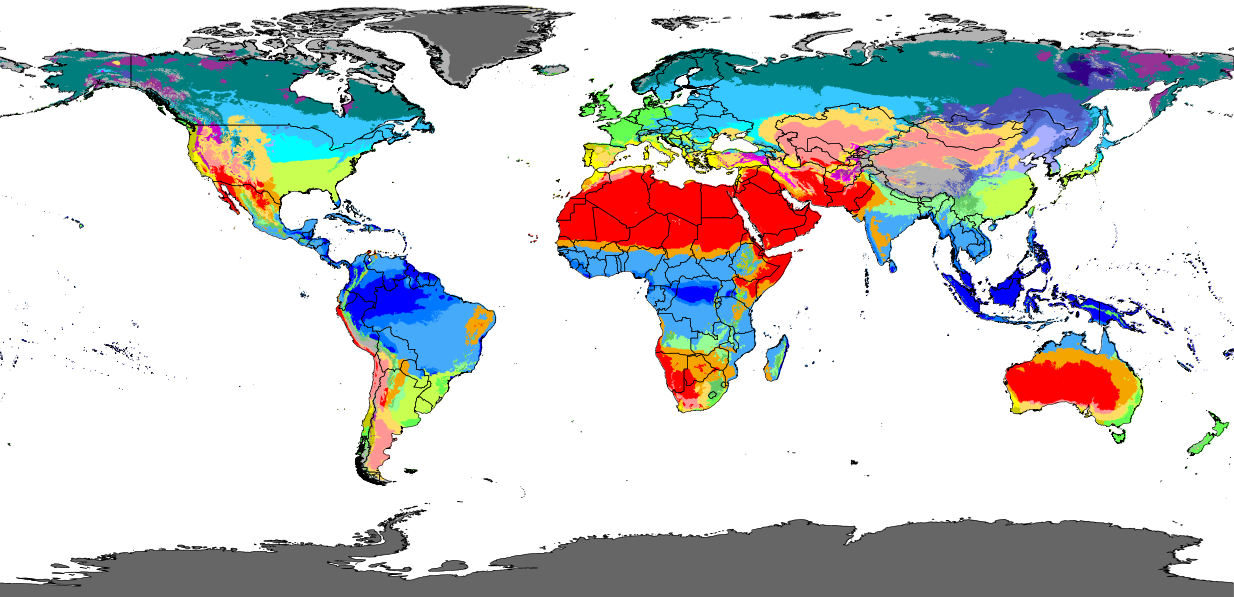
\includegraphics[height=0.3\BenImgWidth]{figures/dataset/KG_Map_cropped.png}};
        \node[anchor=center, font=\scriptsize] (KGMapCap) at ($(KGMap |- LocCap) + (0,0)$) {\textcolor{gray}{Climate}};
        \draw[thin,dotted] ($(PresenceCap.north west) + (0, 0.05)$) -- ($(KGMap.north east |- PresenceCap.west) + (0.05, 0.05)$) -- ($(ClimateLocationTemplate.south east) + (0.05, -.0)$);

        \node[single arrow,minimum height=12mm, minimum width=8mm, single arrow head extend=2mm,
            anchor=west, rotate=90, fill=cyan!90, opacity=0.5] at ($(refMap.north) + (0,-.3)$) {};
        \node[single arrow,minimum height=12mm, minimum width=8mm, single arrow head extend=2mm,
            anchor=west, rotate=0, fill=cyan!90, opacity=0.5] at ($(refMap.east) + (-.3,.4)$) {};
        \node[single arrow,minimum height=12mm, minimum width=8mm, single arrow head extend=2mm,
            anchor=west, rotate=-90, fill=cyan!90, opacity=0.5] at ($(refMap.south) + (0,.3)$) {};
        \node[single arrow,minimum height=10mm, minimum width=8mm, single arrow head extend=2mm,
            anchor=west, rotate=180, fill=cyan!90, opacity=0.5] at ($(refMap.west) + (.3,.4)$) {};

        \node[draw, rounded corners=2mm, thick, dotted, inner sep=4pt, fit=(ClimateLocationTemplate)(SizeCountTemplate), gray!70] (box1) {};

        \node[align=center, anchor=north, text width=99mm, font=\scriptsize] (CombinedTemplates)
            at ($(box1.south) + (0,-0.05)$)
            {
                \colorbox{cyan!20}{This image primary ...  (\textbf{[size]}).}
                \colorbox{WildStrawberry!20}{\textbf{[Class]} is distributed ...  marginal.}
                \colorbox{Dandelion!20}{\textbf{[Class]} is adjacent ... \textbf{[class]}.}
                \colorbox{LimeGreen!20}{The image was ... \textbf{[climate zone]}.}
            };
        \node[draw, rounded corners=2mm, thick, dotted, inner sep=-1pt, fit=(CombinedTemplates), gray!70] (CombinedTemplatesBox) {};
        \node[draw, rounded corners=2mm, thin, dashed, inner sep=1pt, fit=(CombinedTemplatesBox)(box1), gray!90] (TemplatesBox) {};
        \node[inner sep=0pt,minimum size=0pt] (CombineAnchor) at ($(box1.north)!0.5!(CombinedTemplatesBox.south)$) {};
        \node[anchor=center,gray!90, rotate=90, font=\normalsize] at ($(CaptionAnchor |- TemplatesBox)$){\textcolor{gray!90}{\makecell{Extract Attributes,\\Fill \& Concatenate Templates}}};


        \def\scaleLLMRing{0.4}
        \def\LLMRingPointSize{0.05cm}
        \node (baseline_step2_1) at ($(CombinedTemplates.south) + (0,-0.65)$) {};
        \node[anchor=center, draw, circle, minimum size=0.5cm, inner sep=1.5pt, fill=gray!25, font=\tiny] (LLM_paraphrase) at ($(baseline_step2_1) + (-4.15, 0)$) {\scalebox{0.8}{LLM}};
        \node[draw, circle, minimum size=\LLMRingPointSize, inner sep=0pt] (LLM_paraphrase_west) at ($(LLM_paraphrase) + (-\scaleLLMRing,0)$) {};
        \node[draw, circle, minimum size=\LLMRingPointSize, inner sep=0pt] (LLM_paraphrase_east) at ($(LLM_paraphrase) + ( \scaleLLMRing,0)$) {};
        \node[draw, circle, minimum size=\LLMRingPointSize, inner sep=0pt] (LLM_paraphrase_south) at ($(LLM_paraphrase) + (0,-\scaleLLMRing)$) {};
        \node[draw, circle, minimum size=\LLMRingPointSize, inner sep=0pt] (LLM_paraphrase_north) at ($(LLM_paraphrase) + (0, \scaleLLMRing)$) {};
        \node[draw, circle, minimum size=\LLMRingPointSize, inner sep=0pt, fill=black] at ($(LLM_paraphrase) + (-.7070*\scaleLLMRing, .7070*\scaleLLMRing)$) {};
        \node[draw, circle, minimum size=\LLMRingPointSize, inner sep=0pt, fill=black] at ($(LLM_paraphrase) + (-.7070*\scaleLLMRing, -.7070*\scaleLLMRing)$) {};
        \node[draw, circle, minimum size=\LLMRingPointSize, inner sep=0pt, fill=black] at ($(LLM_paraphrase) + (.7070*\scaleLLMRing, .7070*\scaleLLMRing)$) {};
        \node[draw, circle, minimum size=\LLMRingPointSize, inner sep=0pt, fill=black] at ($(LLM_paraphrase) + (.7070*\scaleLLMRing, -.7070*\scaleLLMRing)$) {};
        \centerarc[draw](LLM_paraphrase)(15:30:\scaleLLMRing)
        \centerarc[draw](LLM_paraphrase)(60:75:\scaleLLMRing)
        \centerarc[draw](LLM_paraphrase)(105:120:\scaleLLMRing)
        \centerarc[draw](LLM_paraphrase)(150:165:\scaleLLMRing)
        \centerarc[draw](LLM_paraphrase)(-15:-30:\scaleLLMRing)
        \centerarc[draw](LLM_paraphrase)(-60:-75:\scaleLLMRing)
        \centerarc[draw](LLM_paraphrase)(-105:-120:\scaleLLMRing)
        \centerarc[draw](LLM_paraphrase)(-150:-165:\scaleLLMRing)
        \node[align=justify, anchor=west, text width=80mm, font=\scriptsize] (ParaphrasePrompt)
            at ($(LLM_paraphrase_east.east) + (.1,0)$)
            {\textit{You are a Remote Sensing expert. Use the following definitions to increase variance in the output: ... \\
            Do not violate these rules: ...}};
        \node[draw, rounded corners=2mm, thin, dashed, inner sep=4pt, inner ysep=2pt, fit=(LLM_paraphrase_west)(LLM_paraphrase_north)(LLM_paraphrase_south)(ParaphrasePrompt), gray!90] (box2_1) {};
        \node[anchor=center, gray!90, rotate=90, font=\normalsize] at ($(CaptionAnchor |- box2_1)$) {\textcolor{gray!90}{\makecell{Para-\\phrase}}};

        \node[anchor=center, draw, circle, minimum size=0.5cm, inner sep=1.5pt, fill=gray!25, font=\tiny] (LLM_refine) at ($(LLM_paraphrase) + (0, -1.1)$) {\scalebox{0.8}{LLM}};
        \node[draw, circle, minimum size=\LLMRingPointSize, inner sep=0pt] (LLM_refine_west) at ($(LLM_refine) + (-\scaleLLMRing,0)$) {};
        \node[draw, circle, minimum size=\LLMRingPointSize, inner sep=0pt] (LLM_refine_east)at ($(LLM_refine) + ( \scaleLLMRing,0)$) {};
        \node[draw, circle, minimum size=\LLMRingPointSize, inner sep=0pt] (LLM_refine_south) at ($(LLM_refine) + (0,-\scaleLLMRing)$) {};
        \node[draw, circle, minimum size=\LLMRingPointSize, inner sep=0pt] (LLM_refine_north) at ($(LLM_refine) + (0, \scaleLLMRing)$) {};
        \node[draw, circle, minimum size=\LLMRingPointSize, inner sep=0pt, fill=black] at ($(LLM_refine) + (-.7070*\scaleLLMRing, .7070*\scaleLLMRing)$) {};
        \node[draw, circle, minimum size=\LLMRingPointSize, inner sep=0pt, fill=black] at ($(LLM_refine) + (-.7070*\scaleLLMRing, -.7070*\scaleLLMRing)$) {};
        \node[draw, circle, minimum size=\LLMRingPointSize, inner sep=0pt, fill=black] at ($(LLM_refine) + (.7070*\scaleLLMRing, .7070*\scaleLLMRing)$) {};
        \node[draw, circle, minimum size=\LLMRingPointSize, inner sep=0pt, fill=black] at ($(LLM_refine) + (.7070*\scaleLLMRing, -.7070*\scaleLLMRing)$) {};
        \centerarc[draw](LLM_refine)(15:30:\scaleLLMRing)
        \centerarc[draw](LLM_refine)(60:75:\scaleLLMRing)
        \centerarc[draw](LLM_refine)(105:120:\scaleLLMRing)
        \centerarc[draw](LLM_refine)(150:165:\scaleLLMRing)
        \centerarc[draw](LLM_refine)(-15:-30:\scaleLLMRing)
        \centerarc[draw](LLM_refine)(-60:-75:\scaleLLMRing)
        \centerarc[draw](LLM_refine)(-105:-120:\scaleLLMRing)
        \centerarc[draw](LLM_refine)(-150:-165:\scaleLLMRing)
        \node[align=justify, anchor=west, text width=80mm, font=\scriptsize] (RefinePrompt)
            at ($(LLM_refine_east.east) + (.1,0)$)
            {\textit{Control your caption. Ensure that you followed the rules. Update the caption by ... Do NOT explain the mistakes.}};
        \node[draw, rounded corners=2mm, thin, dashed, inner sep=4pt, inner ysep=2pt, fit=(LLM_refine_west)(LLM_refine_north)(LLM_refine_south)(RefinePrompt), gray!90] (box2_2) {};
        \node[anchor=center,gray!90, rotate=90, font=\normalsize] at ($(CaptionAnchor |- box2_2)$) {\textcolor{gray!90}{\makecell{Refine}}};



        \node[align=justify, anchor=north, text width=108mm, inner sep=2pt, font=\scriptsize] (FinalCaption)
            at ($(box2_2.south) + (0,-0.1)$)
            {This satellite image, captured during the summer season in Switzerland, showcases a diverse landscape within the "temperate, no dry season, warm summer" climate zone. The dominant features are arable land ($\sim$526,000 sqm) and inland wetlands ($\sim$460,000 sqm), which are adjacent to each other. The arable land borders both inland wetlands and urban fabric ($\sim$149,000 sqm). Moreover, the inland wetlands are adjacent to both inland waters ($\sim$305,000 sqm) and urban fabric. Notably, the urban fabric is distributed over three individual marginal areas. The varied landscape presents a mix of agricultural areas, wetlands, water bodies, and artificial surfaces.};
        \node[draw, rounded corners=2mm, thin, dashed, inner sep=0pt, fit=(FinalCaption)($(box2_2.east |- FinalCaption)$)($(box2_2.west |- FinalCaption)$), gray!90] (box3) {};
        \node[anchor=center,gray!90, rotate=90,font=\normalsize] at ($(CaptionAnchor |- box3)$) {\textcolor{gray!90}{\makecell{Final\\Caption}}};

    \end{tikzpicture} 

    \caption{Caption generation process for \bentxt{}: i) Attribute extraction from the reference map and template filling based on the attributes and metadata such as location, season and climate zone information, followed by concatenation of the templates; ii) increasing linguistic variance and ensuring correctness via self-refinement.}
    \label{fig:caption_generation_process}
\end{figure*}
\paragraph{VQA and \genDet{} generation.} We further augment each image pair with question-answer annotations relevant for binary yes/no \ac{VQA}, \ac{MCQ} \ac{VQA}, and \genDet. 
Binary questions target the four spatial categories from the captioning stage (presence, count, size, adjacency), with one \enquote{yes} and one \enquote{no} answer generated per pair. 
To prevent \enquote{no} answers from being solvable by class-absence detection alone, count and size questions are constructed such that the queried class is present but the stated quantity is incorrect; presence and adjacency \enquote{no} questions use semantically similar classes from the \ac{CLC} hierarchy. 
\Acp{MCQ} extend the four spatial categories from the captioning stage with questions about relative class position, acquisition country, season, and Köppen-Geiger climate zone.
Each set of answers for the \acp{MCQ} includes one correct answer and three incorrect ones, sampled by analogous principles to the binary \acp{VQA}. 
For \genDet, we generate \refDet{} instructions targeting instances covering between \SI{1}{\percent} and \SI{50}{\percent} of the image area and at least \SI{40}{\percent} of their enclosing bounding box, along with \pointDet{} instructions for instances whose centroid lies within the instance region. 
Examples are given in \cref{fig:dataset_overview}.
Each annotation type uses more than 20 linguistic templates to ensure variability without relying on \ac{LLM} augmentation. 
In total, each image pair is associated with up to 16 \ac{VQA} pairs, and approximately \SI{80}{\percent} of pairs carry at least one \genDet{} annotation.

\subsection{Caption Statistics\label{sec:statistics}}
The caption annotations of \bentxt{} contain approximately \num{50} million words and \num{2.1} million sentences, averaging 107 words and \num{4.5} sentences. 
The vocabulary comprises \num{12394} unique terms. 
Caption lengths follow a bimodal distribution (\cref{fig:pdf_caption_length}) corresponding to single-class and multi-class scenes: single-class captions are shorter due to the absence of adjacency descriptions, while multi-class captions vary with scene complexity. 
Sentence counts per caption (\cref{fig:pdf_sentences_per_caption}) peak between four and six, reflecting the predominance of complex scenes. 
As shown in \cref{fig:mtld_score}, the caption annotations of \bentxt{} achieve a \ac{MTLD} score of \num{64.69}, surpassing the largest existing image-text \ac{RS} dataset containing images with more than three bands (MS-CLIP~\cite{marimo2025beyond}) by more than $1.7\times$. 
Additionally, caption annotations of \bentxt{} encompass $\sim$\SI{25}{\percent} more words in half as many samples compared to MS-CLIP. This shows that \bentxt{} is not only lexically more diverse, but also richer in the semantic content per caption.
\begin{figure}[h!tb]
\centering
    \subfloat[\notsotiny Length ($\nicefrac{\text{Words}}{\text{Caption}}$)]{
        \raisebox{0mm}{\rotatebox{90}{\hspace{3mm}\textsf{\notsotiny Density of Occurrences}}}
        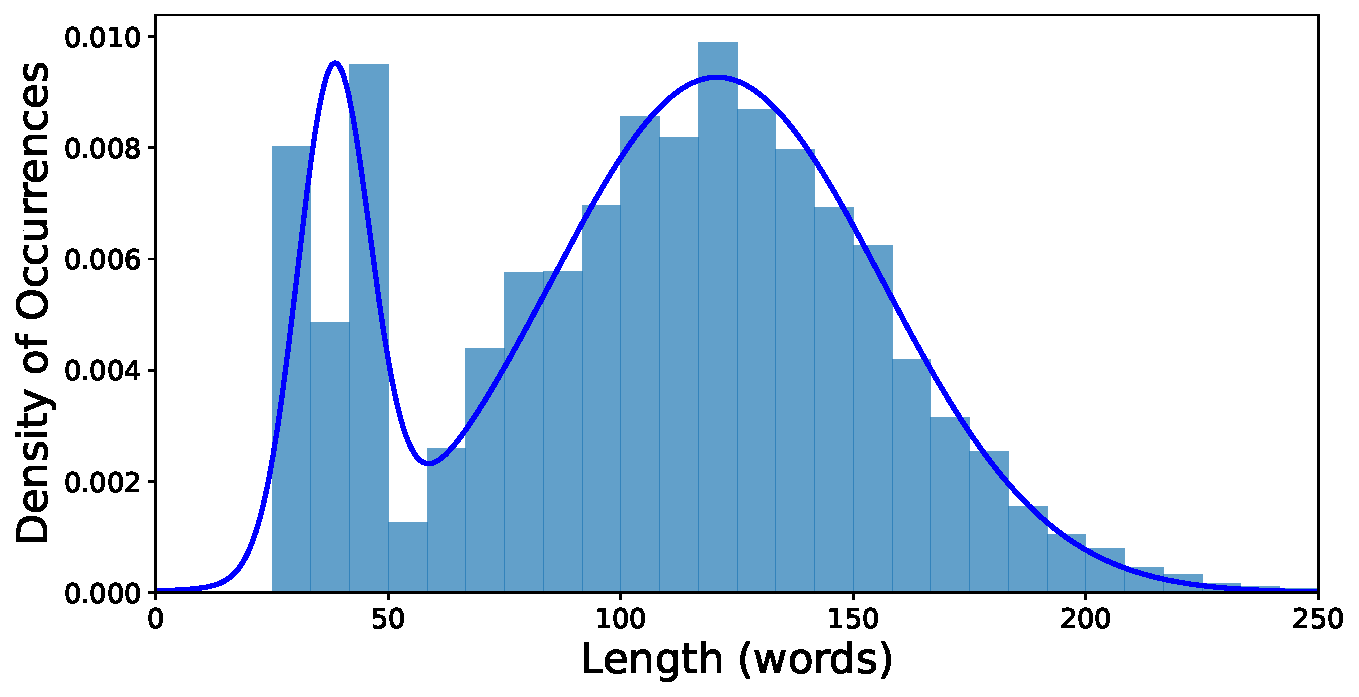
\includegraphics[width=0.44\linewidth,trim=30 32 0 0, clip]{figures/dataset/caption_length_caption_index_2_density.pdf}
        \label{fig:pdf_caption_length}
    }\hfill
    \subfloat[\notsotiny Length ($\nicefrac{\text{Sentences}}{\text{Caption}}$)]{
        \raisebox{0mm}{\rotatebox{90}{\hspace{3mm}\textsf{\notsotiny Density of Occurrences}}}
        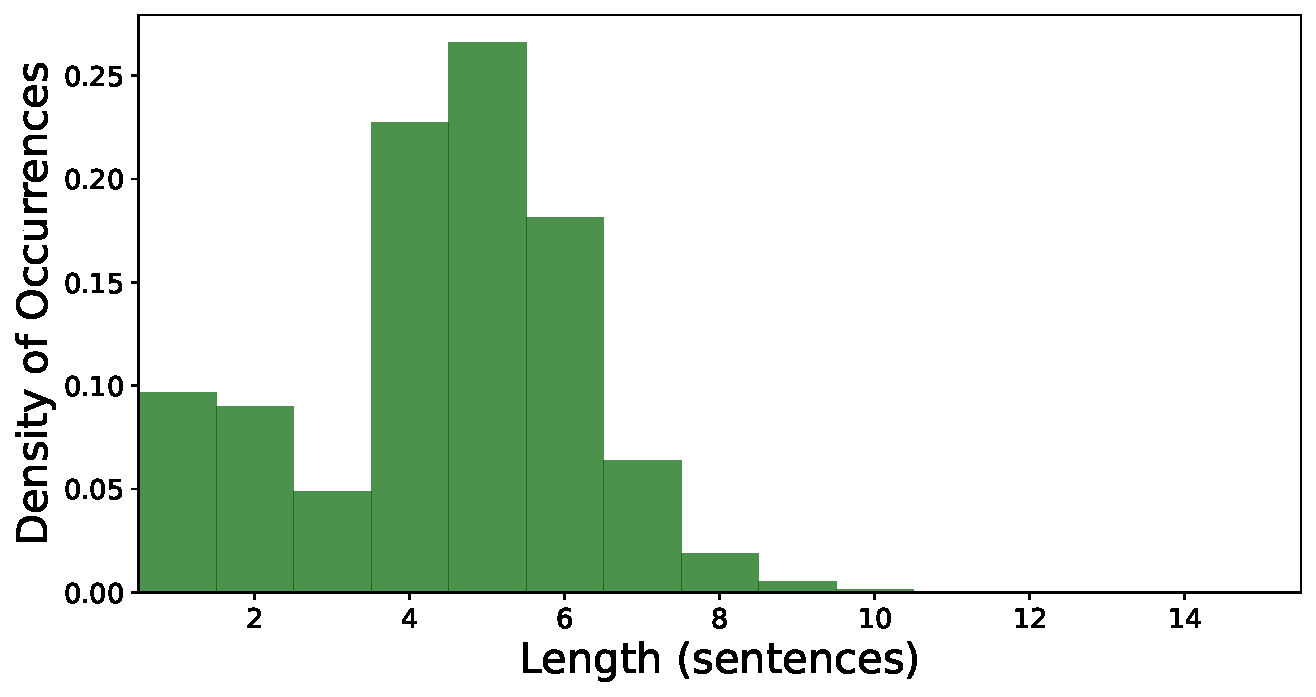
\includegraphics[width=0.44\linewidth,trim=30 32 0 0, clip]{figures/dataset/caption_num_sentences_index_2_density.pdf}
        \label{fig:pdf_sentences_per_caption}
    }\par 
    \subfloat[Number of Image-Text Pairs]{
        \raisebox{0mm}{\rotatebox{90}{\hspace{10mm}\textsf{MTLD Score}}}
        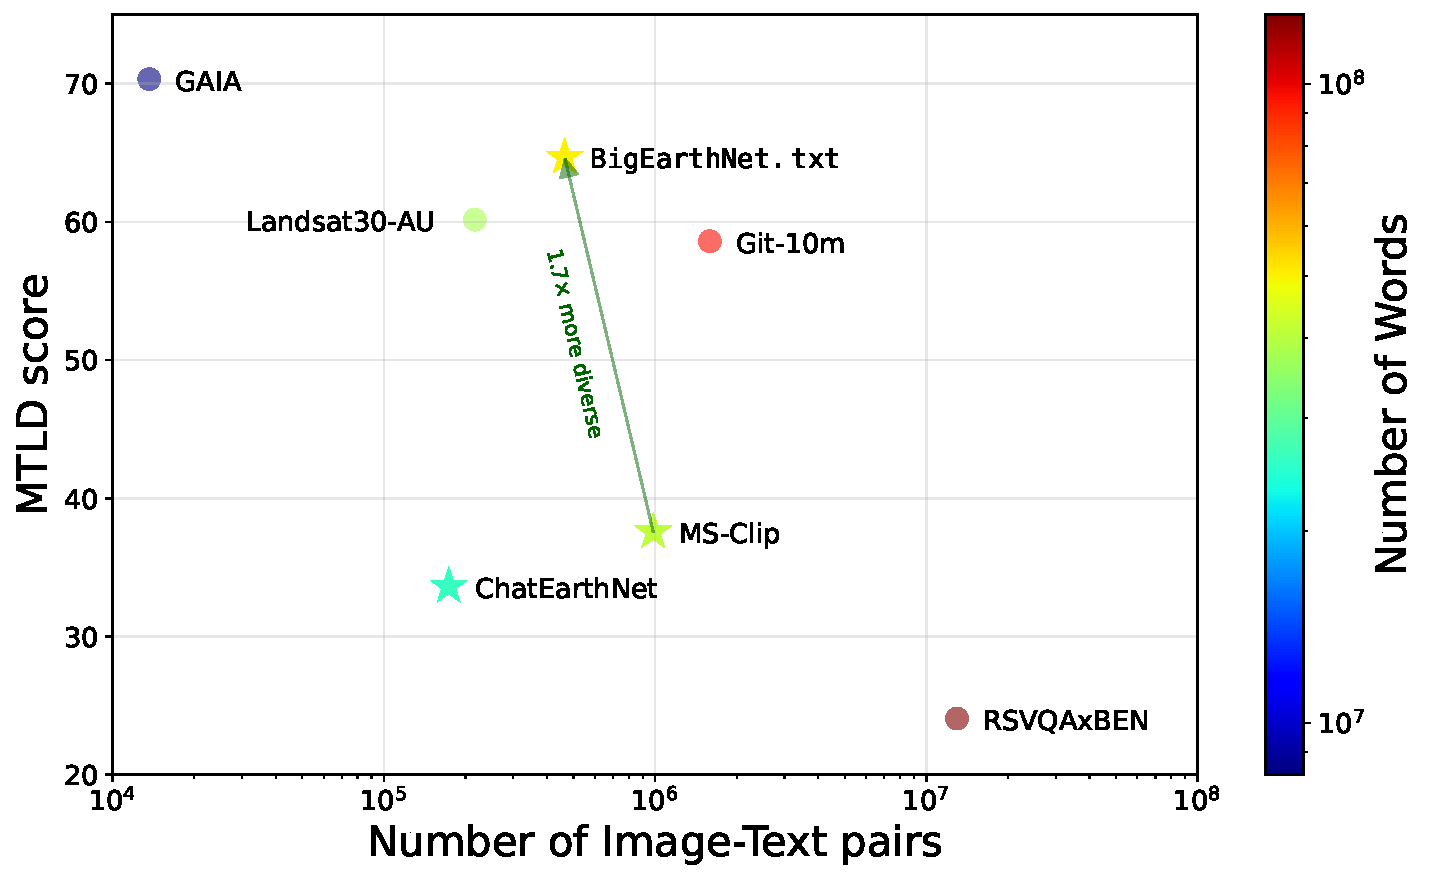
\includegraphics[width=0.45\linewidth,trim=30 30 30 0, clip]{figures/dataset/mtld_score_index_2.pdf}
        \raisebox{0mm}{\rotatebox{90}{\hspace{8mm}\textsf{Number of Words}}}
    \label{fig:mtld_score}
    }
    \caption{\Ac{PDF} of (a) caption lengths and (b) number of sentences in a caption in the \bentxt{} dataset.
     (c) Comparison of existing image-text \ac{RS} datasets in terms of size and semantic richness of the text data. The \ac{NLTK} word tokenizer is used to divide the captions and questions into tokens. The color of each point indicates the total number of tokens in the dataset. Datasets that encompass images with more than three spectral bands are denoted with a star. The \bentxt{} dataset is $1.7\times$ more diverse compared to the largest existing \ac{RS} dataset encompassing more than three bands.}
    \label{fig}
\end{figure}

\subsection{The \bentxt{} \bench{}}

We divide \bentxt{} into train, validation, and test splits as in BigEarthNet~v2.0, resulting in \num{229114}, \num{118095}, and \num{116835} image pairs and \num{4674281}, \num{2454690}, and \num{2424991} text annotations, respectively. However, because LLM-augmented captions may contain hallucinated content, we construct a curated \bench{} to enable reliable model evaluation on the annotations introduced in \bentxt{}. The \bench{} contains \num{1082} image pairs with \num{15029} text annotations from the test split whose augmented captions passed manual verification on all four quality dimensions.
To expose answer-bias in evaluated models, binary and \ac{MCQ} annotations are balanced across answer options.
Annotations are further balanced across \ac{LULC} classes to the extent permitted by their natural distribution. 
Overall, the \bench{} contains \num{6927} binary and \num{5550} multiple-choice \ac{VQA} annotations, \num{970} captions, and \num{1582} \genDet{} annotations across \num{1082} image pairs.